\subsection{Bubble \& eat - Direttore}

\UC{Cancellare ordini al Cuoco}{UC3.12}

\begin{figure}[H]
	\centering
	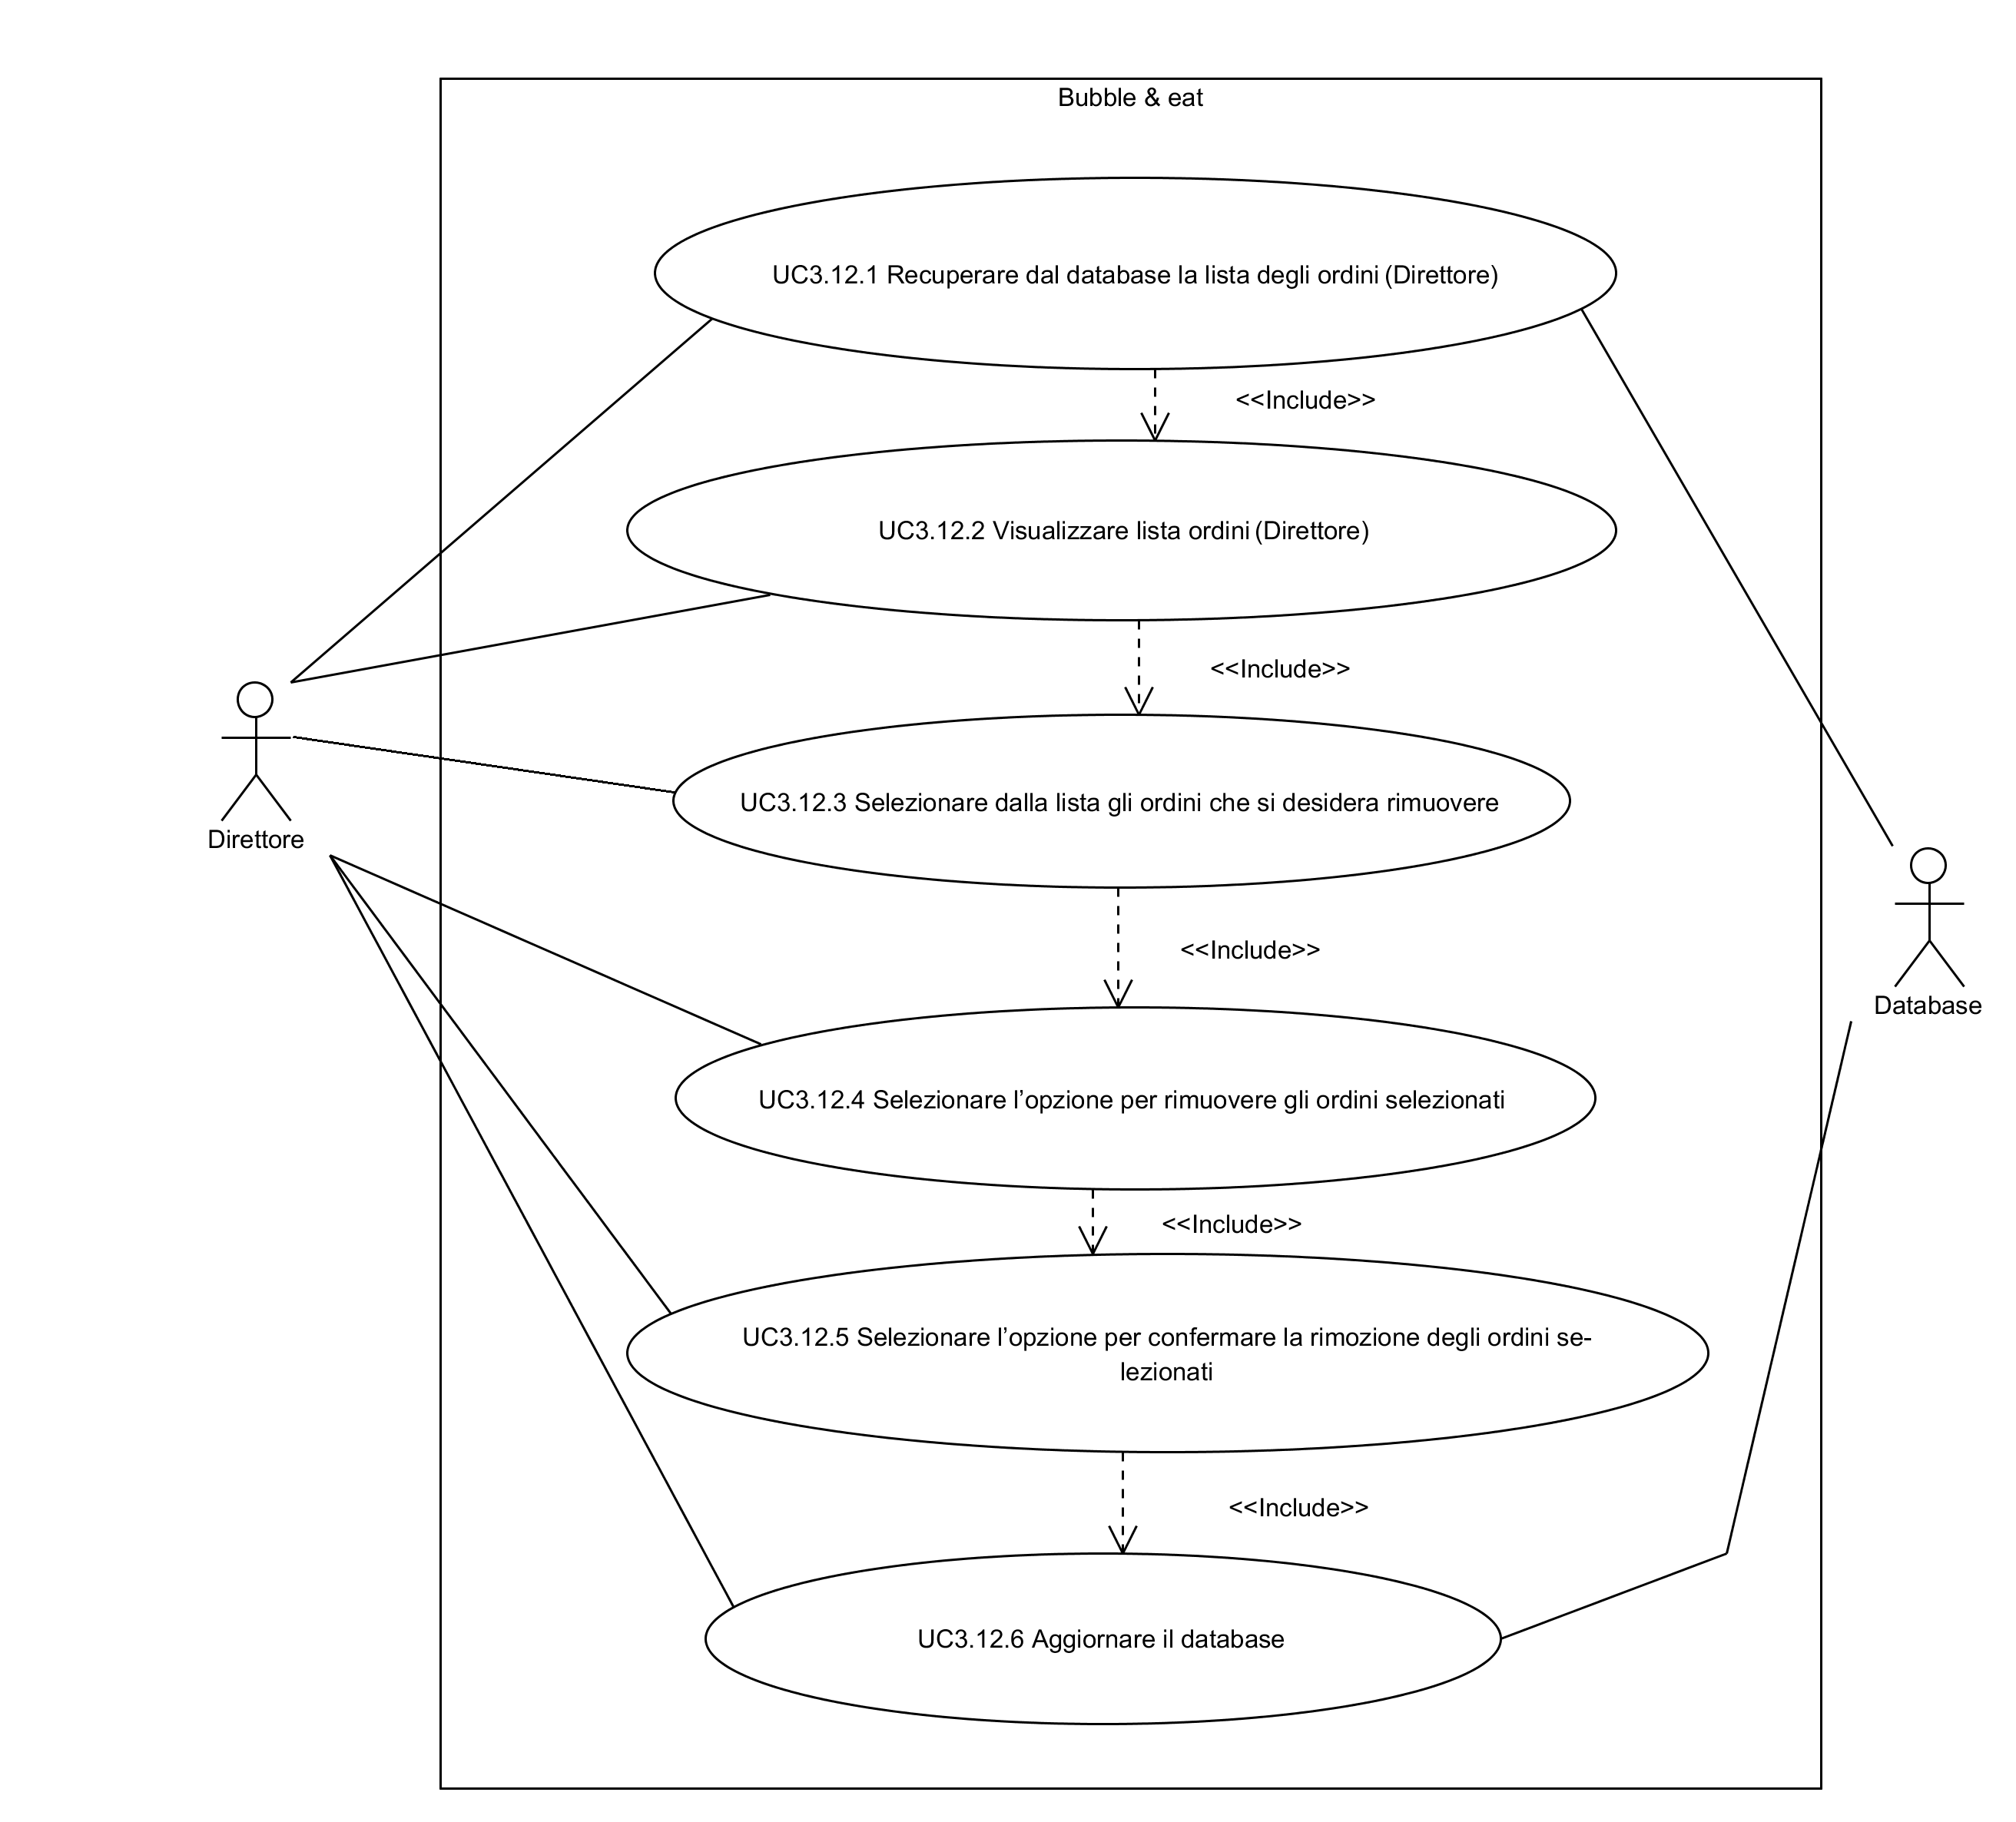
\includegraphics[width=15cm]{../../documenti/AnalisiDeiRequisiti/Diagrammi_img/uc3_12.png}
	\caption{\UCCaption{} Cancellare ordini al Cuoco}
\end{figure}

\begin{itemize}
	\item \textbf{Attori:}
	\\Direttore.
	\item \textbf{Scopo e descrizione:} 
	\\Lo scopo di questa funzione è permettere al Direttore di cancellare ordini dalla to-do list del Cuoco.
	\item \textbf{Precondizioni:}
	\begin{itemize}
		\item Avere Rocket.Chat;
		\item Avere la bubble del ristorante selezionato;
		\item Avere accesso alla bubble con il ruolo di Direttore.
	\end{itemize}
	\item \textbf{Flusso principale degli eventi:}
	\begin{itemize}
		\item Recuperare dal database la lista degli ordini \ref{UC3.12.1};
		\item Visualizzare lista ordini \ref{UC3.12.2};
		\item L'utente Direttore seleziona dalla lista gli ordini che desidera rimuovere \ref{UC3.12.3};
		\item L'utente Direttore seleziona l'opzione per rimuovere gli ordini selezionati \ref{UC3.12.4};
		\item L'utente Direttore seleziona l'opzione per confermare \ref{UC3.12.5};
		\item Aggiornare il database \ref{UC3.12.6}.
	\end{itemize}
	\item \textbf{Post-condizione:}
	\\L'ordine è stato cancellato dalla to-do list del Cuoco.
\end{itemize}

\UCF{Recuperare dal database la lista degli ordini (Direttore)}{UC3.12.1}

\begin{itemize}
	\item \textbf{Attori:}
	\\Direttore.
	\item \textbf{Scopo e descrizione:} 
	\\Lo scopo di questa funzione è permettere alla bubble del Direttore di avere nella propria memoria la lista delle ordinazioni effettuate.
	\item \textbf{Precondizioni:}
	\begin{itemize}
		\item Avere Rocket.Chat;
		\item Avere la bubble del ristorante selezionato;
		\item Avere accesso alla bubble con il ruolo di Direttore.
	\end{itemize}
	\item \textbf{Flusso principale degli eventi:}
	\\Il Direttore consulta la bubble in modalità di cancellazione dell'ordinazione del Cuoco.
	\item \textbf{Post-condizione:}
	\\L'ordine è stato cancellato dalla to-do list del Cuoco.
\end{itemize}

\UCF{Visualizzare lista ordini (Direttore)}{UC3.12.2}

\begin{itemize}
	\item \textbf{Attori:}
	\\Direttore.
	\item \textbf{Scopo e descrizione:} 
	\\Lo scopo di questa funzione è permettere al Direttore di cancellare ordini dalla to-do list del Cuoco.
	\item \textbf{Precondizioni:}
	\begin{itemize}
		\item Avere Rocket.Chat;
		\item Avere la bubble del ristorante selezionato;
		\item Avere accesso alla bubble con il ruolo di Direttore.
	\end{itemize}
	\item \textbf{Flusso principale degli eventi:}
	\\Il Direttore visualizza la lista degli ordini per poterne rimuovere.
	\item \textbf{Post-condizione:}
	\\La lista degli ordini è visualizzata.
\end{itemize}

\UCF{Selezionare dalla lista gli ordini che si desidera rimuovere}{UC3.12.3}

\begin{itemize}
	\item \textbf{Attori:}
	\\Direttore.
	\item \textbf{Scopo e descrizione:} 
	\\Lo scopo di questa funzione è permettere al Direttore di selezionare ordini da cancellare dalla to-do list del Cuoco.
	\item \textbf{Precondizioni:}
	\begin{itemize}
		\item Avere Rocket.Chat;
		\item Avere la bubble del ristorante selezionato;
		\item Avere accesso alla bubble con il ruolo di Direttore;
		\item La lista degli ordini da eliminare è visualizzata.
	\end{itemize}
	\item \textbf{Flusso principale degli eventi:}
	\\Il Direttore sceglie l'ordine da eliminare dalla to-do list del Cuoco.
	\item \textbf{Post-condizione:}
	\\Sono stati selezionati degli ordini dalla lista.
\end{itemize}

\UCF{Selezionare l'opzione per rimuovere gli ordini selezionati}{UC3.12.4}

\begin{itemize}
	\item \textbf{Attori:}
	\\Direttore.
	\item \textbf{Scopo e descrizione:} 
	\\Lo scopo di questa funzione è permettere al Direttore di eliminare gli ordini selezionati per l'eliminazione.
	\item \textbf{Precondizioni:}
	\begin{itemize}
		\item Avere Rocket.Chat;
		\item Avere la bubble del ristorante selezionato;
		\item Avere accesso alla bubble con il ruolo di Direttore;
		\item Sono stati selezionati ordini da eliminare \ref{UC3.12.3}.
	\end{itemize}
	\item \textbf{Flusso principale degli eventi:}
	\\Il Direttore sceglie l'ordine da eliminare dalla to-do list del Cuoco.
	\item \textbf{Post-condizione:}
	\\L'ordine da cancellare è selezionato.
\end{itemize}

\UCF{Selezionare l'opzione per confermare la rimozione degli ordini selezionati}{UC3.12.5}

\begin{itemize}
	\item \textbf{Attori:}
	\\Direttore.
	\item \textbf{Scopo e descrizione:} 
	\\Lo scopo di questa funzione è permettere al Direttore di confermare la selezione degli ordini da eliminare.
	\item \textbf{Precondizioni:}
	\begin{itemize}
		\item Avere Rocket.Chat;
		\item Avere la bubble del ristorante selezionato;
		\item Avere accesso alla bubble con il ruolo di Direttore;
		\item La lista degli ordini da eliminare è visualizzata;
		\item È stata selezionata l'eliminazione degli ordini selezionati \ref{UC3.12.4}.
	\end{itemize}
	\item \textbf{Flusso principale degli eventi:}
	\\Il Direttore sceglie l'ordine da eliminare dalla to-do list del Cuoco.
	\item \textbf{Post-condizione:}
	\\Il Direttore ha confermato quale ordine cancellare.
\end{itemize}

\UCF{Aggiornare il database}{UC3.12.6}

\begin{itemize}
	\item \textbf{Attori:}
	\\Direttore.
	\item \textbf{Scopo e descrizione:} 
	\\Lo scopo di questa funzione è aggiornare il database in base agli ordini cancellati dal Direttore.
	\item \textbf{Precondizioni:}
	\begin{itemize}
		\item Avere Rocket.Chat;
		\item Avere la bubble del ristorante selezionato;
		\item Avere accesso alla bubble con il ruolo di Direttore;
		\item Avere confermato quali ordini eliminare \ref{UC3.12.5}.
	\end{itemize}
	\item \textbf{Flusso principale degli eventi:}
	\\Vengono aggiornati nel database i dati relativi agli ordini da eliminare.
	\item \textbf{Post-condizione:}
	\\L'ordine è stato cancellato dalla to-do list del Cuoco.
\end{itemize}

\UC{Cambiare il menù}{UC3.13}

\begin{figure}[H]
	\centering
	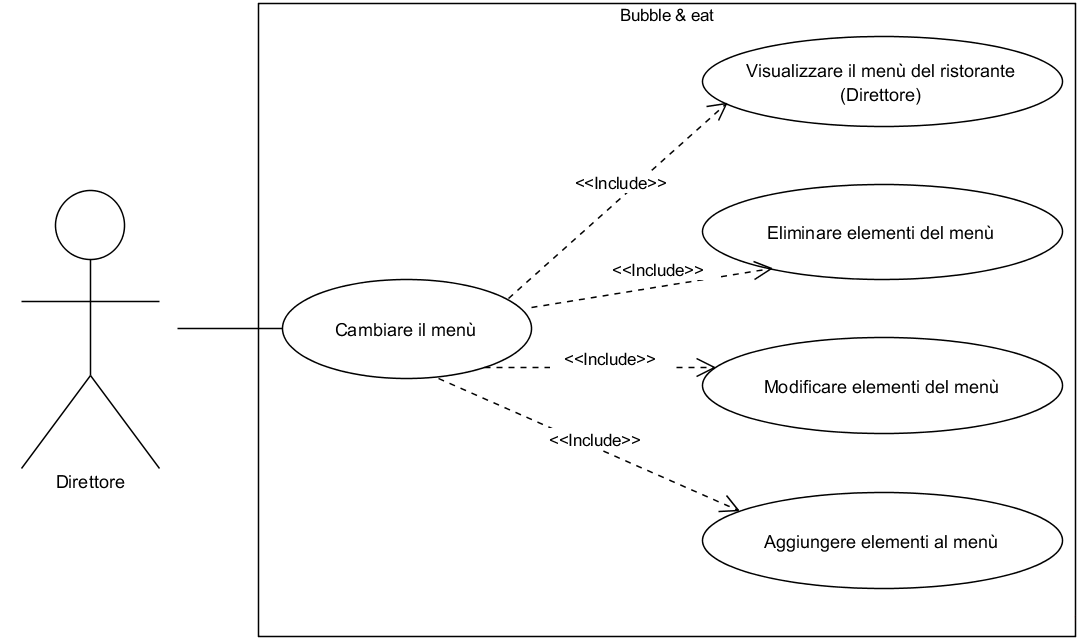
\includegraphics[width=15cm]{../../documenti/AnalisiDeiRequisiti/Diagrammi_img/uc3_13.png}
	\caption{\UCCaption{} Cambiare il menù}
\end{figure}

\begin{itemize}
	\item \textbf{Attori:}
	\\Direttore.
	\item \textbf{Scopo e descrizione:} 
	\\Permettere all'utente Direttore di modificare il menù del ristorante.
	\item \textbf{Precondizioni:}
	\begin{itemize}
		\item Avere Rocket.Chat;
		\item Avere la bubble del ristorante selezionato;
		\item Avere accesso alla bubble con il ruolo di Direttore.
	\end{itemize}
	\item \textbf{Flusso principale degli eventi:}
	\begin{itemize}
		\item Il Direttore visualizza il menù \ref{UC3.13.1};
		\item Il Direttore elimina degli elementi dal menù \ref{UC3.13.2};
		\item Il Direttore modifica degli elementi del menù \ref{UC3.13.3};
		\item Il Direttore aggiunge elementi al menù \ref{UC3.13.4}.
	\end{itemize}
	\item \textbf{Post-condizione:}
	\\Il menù è modificato.
\end{itemize}

\begin{samepage}
\UCF{Visualizzare il menù del ristorante (Direttore)}{UC3.13.1}
\nopagebreak
\begin{figure}[H]
	\centering
	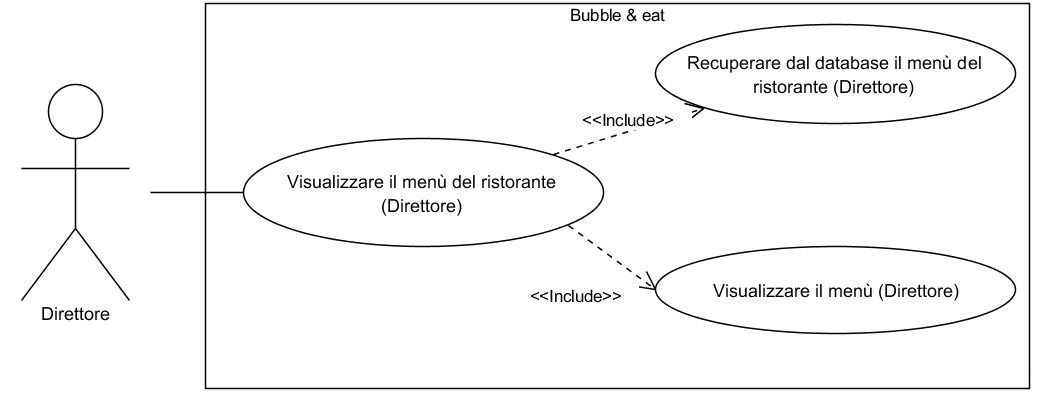
\includegraphics[width=15cm]{../../documenti/AnalisiDeiRequisiti/Diagrammi_img/uc3_13_1.png}
	\caption{\UCFCaption{} Visualizzare il menù del ristorante (Direttore)}
\end{figure}
\end{samepage}

\begin{itemize}
	\item \textbf{Attori:}
	\\Direttore.
	\item \textbf{Scopo e descrizione:} 
	\\Lo scopo di questa funzionalità è di mostrare al Direttore il menù.
	\item \textbf{Precondizioni:}
	\begin{itemize}
		\item Avere Rocket.Chat;
		\item Avere la bubble del ristorante selezionato;
		\item Avere accesso alla bubble con il ruolo di Direttore.
	\end{itemize}
	\item \textbf{Flusso principale degli eventi:}
	\begin{itemize}
		\item Viene recuperato dal database il menù del ristorante \ref{UC3.13.1.1};
		\item Viene mostrato all'utente il menù \ref{UC3.13.1.2}.
	\end{itemize}
	\item \textbf{Post-condizione:}
	\\Nella bubble memory è presente il menù.
\end{itemize}

\UCFF{Recuperare dal database il menù del ristorante (Direttore)}{UC3.13.1.1}

\begin{itemize}
	\item \textbf{Attori:}
	\\Direttore.
	\item \textbf{Scopo e descrizione:} 
	\\Recuperare il menù del ristorante dal database.
	\item \textbf{Precondizioni:}
	\begin{itemize}
		\item Avere Rocket.Chat;
		\item Avere la bubble del ristorante selezionato;
		\item Avere accesso alla bubble con il ruolo di Direttore.
	\end{itemize}
	\item \textbf{Flusso principale degli eventi:}
	\\Il Direttore accede alla sezione di modifica del menù della sua bubble.
	\item \textbf{Post-condizione:}
	\\Nella bubble memory è presente il menù.
\end{itemize}

\UCFF{Visualizzare il menù (Direttore)}{UC3.13.1.2}

\begin{itemize}
	\item \textbf{Attori:}
	\\Direttore.
	\item \textbf{Scopo e descrizione:} 
	\\Il Direttore deve poter visualizzare il menù per poterlo modificare.
	\item \textbf{Precondizioni:}
	\begin{itemize}
		\item Avere Rocket.Chat;
		\item Avere la bubble del ristorante selezionato;
		\item Avere accesso alla bubble con il ruolo di Direttore;
		\item Aver recuperato le informazioni dal database \ref{UC3.13.1.1}.
	\end{itemize}
	\item \textbf{Flusso principale degli eventi:}
	\\Il Direttore si trova nel menù.
	\item \textbf{Post-condizione:}
	\\Il menù è visualizzato.
\end{itemize}

\begin{samepage}
\UCF{Eliminare elementi dal menù}{UC3.13.2}
\nopagebreak
\begin{figure}[H]
	\centering
	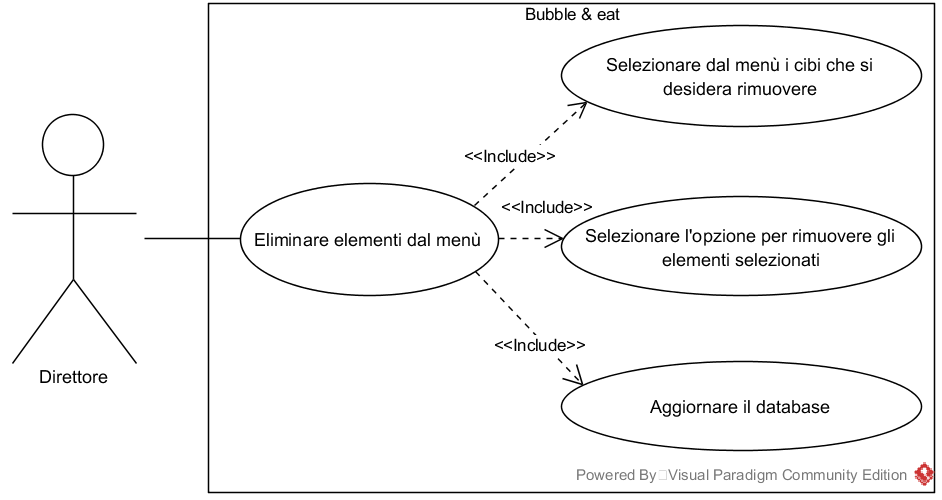
\includegraphics[width=15cm]{../../documenti/AnalisiDeiRequisiti/Diagrammi_img/uc3_13_2.png}
	\caption{\UCFCaption{} Eliminare elementi dal menù}
\end{figure}
\end{samepage}

\begin{itemize}
	\item \textbf{Attori:}
	\\Direttore.
	\item \textbf{Scopo e descrizione:} 
	\\Lo scopo di questa funzionalità è di eliminare elementi dal menù.
	\item \textbf{Precondizioni:}
	\begin{itemize}
		\item Avere Rocket.Chat;
		\item Avere la bubble del ristorante selezionato;
		\item Avere accesso alla bubble con il ruolo di Direttore;
		\item Aver visualizzato il menù del ristorante \ref{UC3.13.1}.
	\end{itemize}
	\item \textbf{Flusso principale degli eventi:}
	\begin{itemize}
		\item Il Direttore seleziona dal menù i cibi che desidera togliere \ref{UC3.13.2.1};
		\item Il Direttore conferma l'operazione \ref{UC3.13.2.2};
		\item Il database viene aggiornato \ref{UC3.13.2.3}.
	\end{itemize}
	\item \textbf{Post-condizione:}
	\\Gli elementi desiderati sono stati eliminati dal menù.
\end{itemize}

\UCFF{Selezionare dal menù i cibi che si desidera rimuovere}{UC3.13.2.1}

\begin{itemize}
	\item \textbf{Attori:}
	\\Direttore.
	\item \textbf{Scopo e descrizione:} 
	\\Avere una selezione di voci da rimuovere dal menù.
	\item \textbf{Precondizioni:}
	\begin{itemize}
		\item Avere Rocket.Chat;
		\item Avere la bubble del ristorante selezionato;
		\item Avere accesso alla bubble con il ruolo di Direttore;
		\item Aver visualizzato il menù del ristorante \ref{UC3.13.1}.
	\end{itemize}
	\item \textbf{Flusso principale degli eventi:}
	\\Il Direttore seleziona dalla lista visualizzata in \ref{UC3.13.1} gli elementi del menù che desidera rimuovere da esso.
	\item \textbf{Post-condizione:}
	\\Gli elementi sono stati selezionati.
\end{itemize}

\UCFF{Selezionare l'opzione per rimuovere gli elementi selezionati}{UC3.13.2.2}

\begin{itemize}
	\item \textbf{Attori:}
	\\Direttore.
	\item \textbf{Scopo e descrizione:} 
	\\Rimuovere gli elementi selezionati con l'apposita opzione.
	\item \textbf{Precondizioni:}
	\begin{itemize}
		\item Avere Rocket.Chat;
		\item Avere la bubble del ristorante selezionato;
		\item Avere accesso alla bubble con il ruolo di Direttore;
		\item Aver visualizzato il menù del ristorante \ref{UC3.13.1}.
	\end{itemize}
	\item \textbf{Flusso principale degli eventi:}
	\\Il Direttore si trova nel menù, ha selezionato gli elementi da eliminare, e ne conferma l'eliminazione.
	\item \textbf{Post-condizione:}
	\\Gli elementi sono eliminati dal menù.
\end{itemize}

\UCFF{Aggiornare il database}{UC3.13.2.3}

\begin{itemize}
	\item \textbf{Attori:}
	\\Direttore.
	\item \textbf{Scopo e descrizione:} 
	\\Notificare al sistema l'aggiornamento del menù effettuato allo \ref{UC3.13.2.2}.
	\item \textbf{Precondizioni:}
	\begin{itemize}
		\item Avere Rocket.Chat;
		\item Avere la bubble del ristorante selezionato;
		\item Avere accesso alla bubble con il ruolo di Direttore;
		\item Aver selezionato l'opzione per rimuovere gli elementi selezionati dal menù \ref{UC3.13.2.2}.
	\end{itemize}
	\item \textbf{Flusso principale degli eventi:}
	\\Il Direttore ha confermato l'eliminazione dal menù degli elementi selezionati in precedenza.
	\item \textbf{Post-condizione:}
	\\La modifica del menù è stata propagata al database.
\end{itemize}

\begin{samepage}
\UCF{Modificare elementi del menù}{UC3.13.3}
\nopagebreak
\begin{figure}[H]
	\centering
	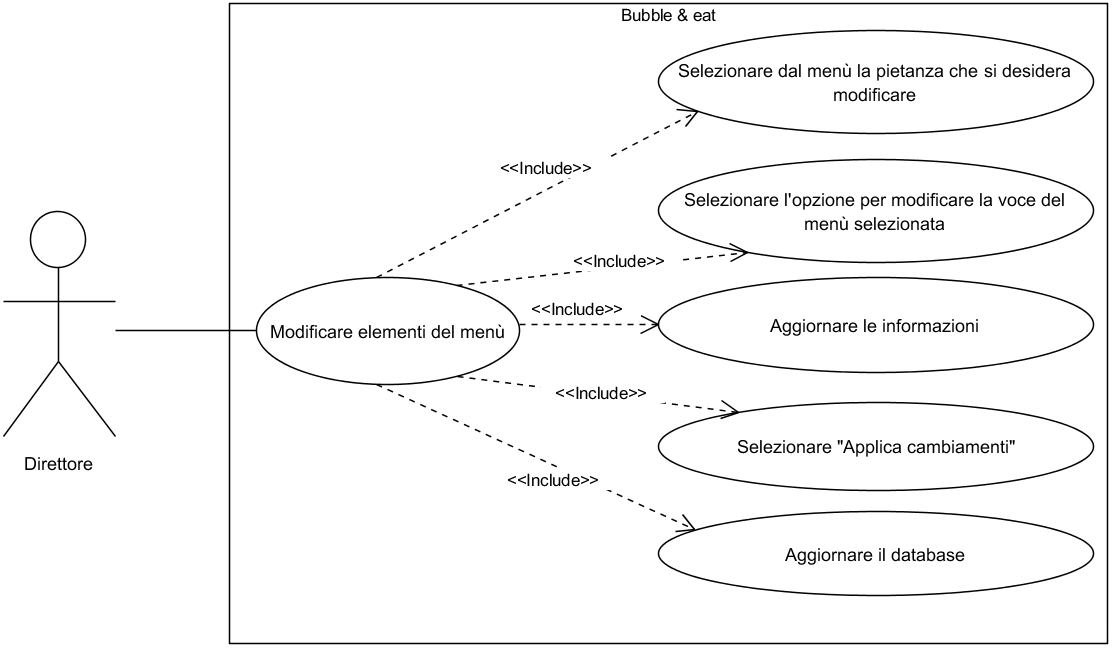
\includegraphics[width=15cm]{../../documenti/AnalisiDeiRequisiti/Diagrammi_img/uc3_13_3.png}
	\caption{\UCFCaption{} Modificare elementi del menù}
\end{figure}
\end{samepage}

\begin{itemize}
	\item \textbf{Attori:}
	\\Direttore.
	\item \textbf{Scopo e descrizione:} 
	\\Lo scopo di questa funzionalità è di permettere al Direttore di modificare elementi del menù.
	\item \textbf{Precondizioni:}
	\begin{itemize}
		\item Avere Rocket.Chat;
		\item Avere la bubble del ristorante selezionato;
		\item Avere accesso alla bubble con il ruolo di Direttore;
		\item Aver visualizzato il menù del ristorante \ref{UC3.13.1}.
	\end{itemize}
	\item \textbf{Flusso principale degli eventi:}
	\begin{itemize}
		\item Il Direttore seleziona dal menù l'elemento che desidera modificare \ref{UC3.13.3.1};
		\item Viene confermata la selezione \ref{UC3.13.3.2};
		\item Il Direttore inserisce le nuove informazioni \ref{UC3.13.3.3};
		\item Vengono confermati i cambiamenti \ref{UC3.13.3.4};
		\item Il database viene aggiornato \ref{UC3.13.3.5}.
	\end{itemize}
	\item \textbf{Post-condizione:}
	\\Sono state applicate le modifiche desiderate agli elementi del menù.
\end{itemize}

\UCFF{Selezionare dal menù il cibo che si desidera modificare}{UC3.13.3.1}

\begin{itemize}
	\item \textbf{Attori:}
	\\Direttore.
	\item \textbf{Scopo e descrizione:} 
	\\Permettere all'utente Direttore di modificare voci del menù.
	\item \textbf{Precondizioni:}
	\begin{itemize}
		\item Avere Rocket.Chat;
		\item Avere la bubble del ristorante selezionato;
		\item Avere accesso alla bubble con il ruolo di Direttore.
	\end{itemize}
	\item \textbf{Flusso principale degli eventi:}
	\\Il Direttore si trova nel menù, può selezionare la voce del menù da modificare.
	\item \textbf{Post-condizione:}
	\\Le voci sono selezionate.
\end{itemize}

\UCFF{Selezionare l'opzione per modificare la voce del menù selezionata}{UC3.13.3.2}

\begin{itemize}
	\item \textbf{Attori:}
	\\Direttore.
	\item \textbf{Scopo e descrizione:} 
	\\Abilitare il cambiamento della voce del menù selezionata.
	\item \textbf{Precondizioni:}
	\begin{itemize}
		\item Avere Rocket.Chat;
		\item Avere la bubble del ristorante selezionato;
		\item Avere accesso alla bubble con il ruolo di Direttore;
		\item Aver visualizzato il menù del ristorante \ref{UC3.13.1}.
	\end{itemize}
	\item \textbf{Flusso principale degli eventi:}
	\\Il Direttore utilizza l'apposito comando per modificare la voce del menù selezionata al caso d'uso \ref{UC3.13.3.1}.
	\item \textbf{Post-condizione:}
	\\La modifica alla voce del menù selezionata è ora disponibile.
\end{itemize}

\UCFF{Aggiornare le informazioni}{UC3.13.3.3}

\begin{itemize}
	\item \textbf{Attori:}
	\\Direttore.
	\item \textbf{Scopo e descrizione:} 
	\\Modificare le informazioni della voce di menù appena selezionata.
	\item \textbf{Precondizioni:}
	\begin{itemize}
		\item Avere Rocket.Chat;
		\item Avere la bubble del ristorante selezionato;
		\item Avere accesso alla bubble con il ruolo di Direttore;
		\item Aver selezionato una voce da modificare.
	\end{itemize}
	\item \textbf{Flusso principale degli eventi:}
	\\Il Direttore può modificare i dati della voce appena selezionata.
	\item \textbf{Post-condizione:}
	\\I dati della voce di menù sono modificati.
\end{itemize}

\UCFF{Selezionare \virgolette{Applica cambiamenti}}{UC3.13.3.4}

\begin{itemize}
	\item \textbf{Attori:}
	\\Direttore.
	\item \textbf{Scopo e descrizione:} 
	\\Applicare i cambiamenti effettuati.
	\item \textbf{Precondizioni:}
	\begin{itemize}
		\item Avere Rocket.Chat;
		\item Avere la bubble del ristorante selezionato;
		\item Avere accesso alla bubble con il ruolo di Direttore;
		\item Aver effettuato delle modifiche sul menù.
	\end{itemize}
	\item \textbf{Flusso principale degli eventi:}
	\\Il Direttore dopo aver finito di applicare tutti i cambiamenti desiderati al menù seleziona l'opzione \virgolette{Applica cambiamenti}; i cambiamenti vengono dunque memorizzati all'interno della bubble.
	\item \textbf{Post-condizione:}
	\\I cambiamenti sono stati applicati e memorizzati all'interno della bubble.
\end{itemize}

\UCFF{Aggiornare il database con le nuove informazioni}{UC3.13.3.5}

\begin{itemize}
	\item \textbf{Attori:}
	\\Direttore.
	\item \textbf{Scopo e descrizione:} 
	\\Propagare nel database le modifiche effettuate nello \ref{UC3.13.3}.
	\item \textbf{Precondizioni:}
	\begin{itemize}
		\item Avere Rocket.Chat;
		\item Avere la bubble del ristorante selezionato;
		\item Avere accesso alla bubble con il ruolo di Direttore;
		\item Aver selezionato \virgolette{Applica cambiamenti} \ref{UC3.13.4}.
	\end{itemize}
	\item \textbf{Flusso principale degli eventi:}
	\\Le modifiche confermate dal Direttore vengono salvate sul database.
	\item \textbf{Post-condizione:}
	\\Il menù è modificato.
\end{itemize}

\begin{samepage}
\UCF{Aggiungere elementi al menù}{UC3.13.4}
\nopagebreak
\begin{figure}[H]
	\centering
	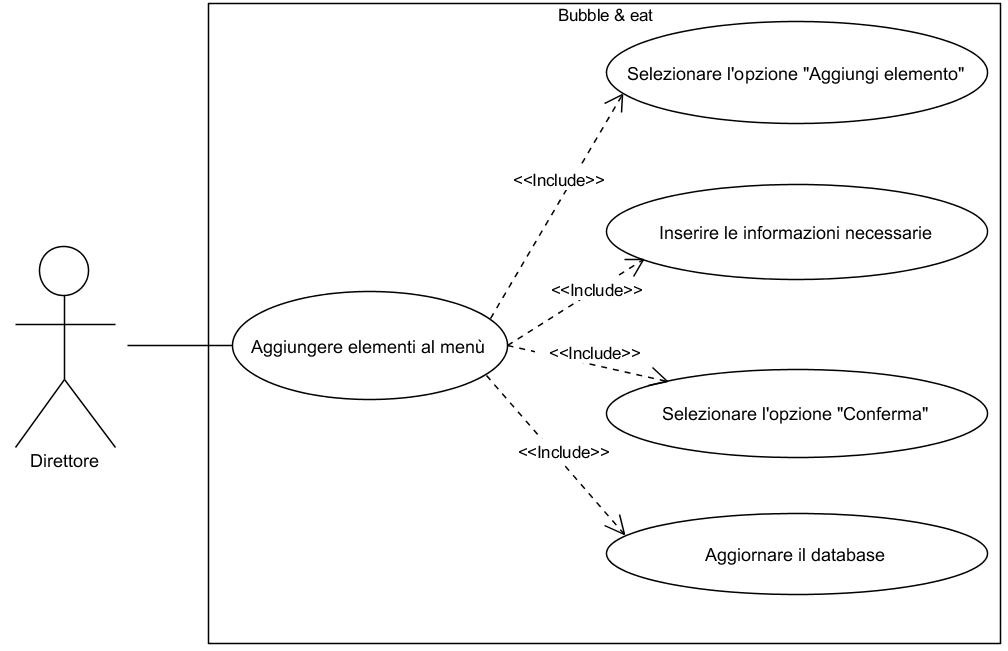
\includegraphics[width=15cm]{../../documenti/AnalisiDeiRequisiti/Diagrammi_img/uc3_13_4.png}
	\caption{\UCFCaption{} Aggiungere elementi al menù}
\end{figure}
\end{samepage}

\begin{itemize}
	\item \textbf{Attori:}
	\\Direttore.
	\item \textbf{Scopo e descrizione:} 
	\\Lo scopo di questa funzionalità è di permettere al Direttore di aggiungere elementi al menù.
	\item \textbf{Precondizioni:}
	\begin{itemize}
		\item Avere Rocket.Chat;
		\item Avere la bubble del ristorante selezionato;
		\item Avere accesso alla bubble con il ruolo di Direttore;
		\item Aver visualizzato il menù del ristorante \ref{UC3.13.1}.
	\end{itemize}
	\item \textbf{Flusso principale degli eventi:}
	\begin{itemize}
		\item Il Direttore seleziona l'opzione per aggiungere un elemento \ref{UC3.13.4.1};
		\item Vengono inserite le informazioni necessarie alla creazione del nuovo elemento \ref{UC3.13.4.2};
		\item Il Direttore conferma l'aggiunta del nuovo elemento \ref{UC3.13.4.3};
		\item Il database viene aggiornato \ref{UC3.13.4.4}.
	\end{itemize}
	\item \textbf{Post-condizione:}
	\\È stato aggiunto un elemento al menù.
\end{itemize}

\UCFF{Selezionare l'opzione \virgolette{Aggiungi elemento}}{UC3.13.4.1}

\begin{itemize}
	\item \textbf{Attori:}
	\\Direttore.
	\item \textbf{Scopo e descrizione:} 
	\\Permettere al Direttore di aggiungere una voce al menù.
	\item \textbf{Precondizioni:}
	\begin{itemize}
		\item Avere Rocket.Chat;
		\item Avere la bubble del ristorante selezionato;
		\item Avere accesso alla bubble con il ruolo di Direttore;
		\item Il menù deve essere visualizzato.
	\end{itemize}
	\item \textbf{Flusso principale degli eventi:}
	\\Il Direttore si trova nel menù, seleziona l'apposita opzione \virgolette{Aggiungi elemento}.
	\item \textbf{Post-condizione:}
	\\È possibile aggiungere i dati per la nuova voce.
\end{itemize}

\UCFF{Inserire le informazioni necessarie}{UC3.13.4.2}

\begin{itemize}
	\item \textbf{Attori:}
	\\Direttore.
	\item \textbf{Scopo e descrizione:} 
	\\Lo scopo di questa funzionalità è quello di permettere al Direttore di inserire le informazioni necessarie all'aggiunta di un elemento al menù.
	\item \textbf{Precondizioni:}
	\begin{itemize}
		\item Avere Rocket.Chat;
		\item Avere la bubble del ristorante selezionato;
		\item Avere accesso alla bubble con il ruolo di Direttore;
		\item Aver iniziato la procedura di aggiunta di un elemento come da \ref{UC3.13.4.1}.
	\end{itemize}
	\item \textbf{Flusso principale degli eventi:}
	\\Il Direttore compila il form caricato dalla bubble in tutte le sue parti.
	\item \textbf{Post-condizione:}
	\\Il Direttore ha inserito all'interno del form tutte le informazioni necessarie ad aggiungere un elemento al menù.
\end{itemize}

\UCFF{Selezionare l'opzione \virgolette{Conferma}}{UC3.13.4.3}

\begin{itemize}
	\item \textbf{Attori:}
	\\Direttore.
	\item \textbf{Scopo e descrizione:} 
	\\Lo scopo di questa funzionalità è quello di permettere al Direttore di inserire le informazioni necessarie all'aggiunta di un elemento al menù.
	\item \textbf{Precondizioni:}
	\begin{itemize}
		\item Avere Rocket.Chat;
		\item Avere la bubble del ristorante selezionato;
		\item Avere accesso alla bubble con il ruolo di Direttore;
		\item Aver inserito le informazioni necessarie \ref{UC3.13.4.2}.
	\end{itemize}
	\item \textbf{Flusso principale degli eventi:}
	\\Il Direttore conferma le modifiche al menù.
	\item \textbf{Post-condizione:}
	\\Le modifiche sono state confermate e sono pronte per l'invio al database.
\end{itemize}

\UCFF{Aggiornare il database con le nuove informazioni}{UC3.13.4.4}

\begin{itemize}
	\item \textbf{Attori:}
	\\Direttore.
	\item \textbf{Scopo e descrizione:} 
	\\Propagare nel database le modifiche effettuate in \ref{UC3.13.4}.
	\item \textbf{Precondizioni:}
	\begin{itemize}
		\item Avere Rocket.Chat;
		\item Avere la bubble del ristorante selezionato;
		\item Avere accesso alla bubble con il ruolo di Direttore;
		\item Aver confermato l'aggiunta \ref{UC3.13.4.3}.
	\end{itemize}
	\item \textbf{Flusso principale degli eventi:}
	\\Le modifiche confermate dal Direttore vengono propagate al database.
	\item \textbf{Post-condizione:}
	\\Il menù è modificato e la modifica è presente anche nel database.
\end{itemize}

\UC{Aggiungere ordini al Responsabile Acquisti}{UC3.14}

\begin{figure}[H]
	\centering
	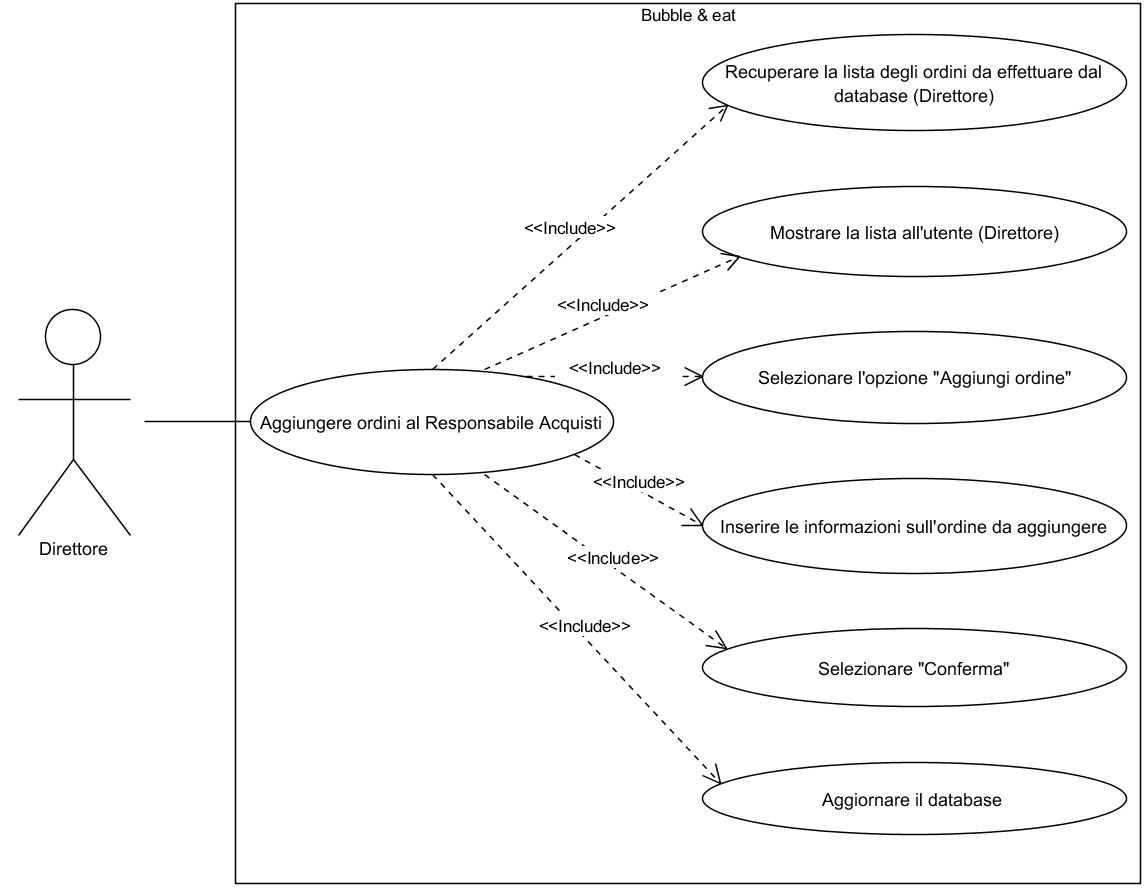
\includegraphics[width=15cm]{../../documenti/AnalisiDeiRequisiti/Diagrammi_img/uc3_14.png}
	\caption{\UCCaption{} Aggiungere ordini al Responsabile Acquisti}
\end{figure}

\begin{itemize}
	\item \textbf{Attori:}
	\\Direttore.
	\item \textbf{Scopo e descrizione:} 
	\\Lo scopo di questa funzione è permettere al Direttore di aggiungere ordini alla to-do list del Responsabile Acquisti.
	\item \textbf{Precondizioni:}
	\begin{itemize}
		\item Avere Rocket.Chat;
		\item Avere la bubble del ristorante selezionato;
		\item Avere accesso alla bubble con il ruolo di Direttore.
	\end{itemize}
	\item \textbf{Flusso principale degli eventi:}
	\begin{itemize}
		\item Recuperare la lista degli ordini da effettuare dal database \ref{UC3.14.1};
		\item Mostrare la lista all'utente \ref{UC3.14.2};
		\item L'utente Direttore seleziona \virgolette{Aggiungi ordine} \ref{UC3.14.3};
		\item L'utente Direttore inserisce le informazioni sull'ordine da aggiungere \ref{UC3.14.4};
		\item L'utente Direttore seleziona \virgolette{Conferma} \ref{UC3.14.5};
		\item Aggiornare il database \ref{UC3.14.6}.
	\end{itemize}
	\item \textbf{Post-condizione:}
	\\Il Direttore ha aggiunto gli elementi desiderati alla to-do list del Responsabile Acquisti.
\end{itemize}

\UCF{Recuperare la lista degli ordini da effettuare dal database (Direttore)}{UC3.14.1}

\begin{itemize}
	\item \textbf{Attori:}
	\\Direttore.
	\item \textbf{Scopo e descrizione:} 
	\\Lo scopo di questa funzione è recuperare le informazioni sulla lista di ordini da effettuare dal database.
	\item \textbf{Precondizioni:}
	\begin{itemize}
		\item Avere Rocket.Chat;
		\item Avere la bubble del ristorante selezionato;
		\item Avere accesso alla bubble con il ruolo di Direttore.
	\end{itemize}
	\item \textbf{Flusso principale degli eventi:}
	\\I dati sugli ordini da effettuare devono essere prelevati dal database.
	\item \textbf{Post-condizione:}
	\\I dati sono prelevati dal database.
\end{itemize}

\UCF{Mostrare la lista all'utente (Direttore)}{UC3.14.2}

\begin{itemize}
	\item \textbf{Attori:}
	\\Direttore.
	\item \textbf{Scopo e descrizione:} 
	\\Lo scopo di questa funzione è permettere al Direttore di visualizzare la lista degli ordini da effettuare.
	\item \textbf{Precondizioni:}
	\begin{itemize}
		\item Avere Rocket.Chat;
		\item Avere la bubble del ristorante selezionato;
		\item Avere accesso alla bubble con il ruolo di Direttore;
		\item Aver recuperato dal database le informazioni \ref{UC3.14.1}.
	\end{itemize}
	\item \textbf{Flusso principale degli eventi:}
	\\Il Direttore deve visualizzare la lista degli ordini da effettuare.
	\item \textbf{Post-condizione:}
	\\La lista è visualizzata.
\end{itemize}

\UCF{Selezionare l'opzione \virgolette{Aggiungi ordine}}{UC3.14.3}

\begin{itemize}
	\item \textbf{Attori:}
	\\Direttore.
	\item \textbf{Scopo e descrizione:} 
	\\Lo scopo di questa funzione è permettere al Direttore di selezionare l'opzione per aggiungere ordini alla to-do list del Responsabile Acquisti.
	\item \textbf{Precondizioni:}
	\begin{itemize}
		\item Avere Rocket.Chat;
		\item Avere la bubble del ristorante selezionato;
		\item Avere accesso alla bubble con il ruolo di Direttore;
		\item La lista degli ordini da effettuare è visualizzata \ref{UC3.14.2}.
	\end{itemize}
	\item \textbf{Flusso principale degli eventi:}
	\\Il Direttore seleziona l'opzione per aggiungere un ordine.
	\item \textbf{Post-condizione:}
	\\Il Direttore ha selezionato \virgolette{Aggiungi ordine}.
\end{itemize}

\UCF{Inserire le informazioni sull'ordine da aggiungere}{UC3.14.4}

\begin{itemize}
	\item \textbf{Attori:}
	\\Direttore.
	\item \textbf{Scopo e descrizione:} 
	\\Lo scopo di questa funzione è permettere al Direttore di aggiungere informazioni all'ordine da aggiungere alla to-do list del Responsabile Acquisti.
	\item \textbf{Precondizioni:}
	\begin{itemize}
		\item Avere Rocket.Chat;
		\item Avere la bubble del ristorante selezionato;
		\item Avere accesso alla bubble con il ruolo di Direttore;
		\item Aver selezionato l'opzione \virgolette{Aggiungi ordine} \ref{UC3.14.3}.
	\end{itemize}
	\item \textbf{Flusso principale degli eventi:}
	\\Il Direttore aggiunge informazioni agli elementi da ordinare desiderati per la to-do list del Responsabile Acquisti.
	\item \textbf{Post-condizione:}
	\\Le informazioni sull'ordine possono essere aggiunte.
\end{itemize}

\UCF{Selezionare \virgolette{Conferma}}{UC3.14.5}

\begin{itemize}
	\item \textbf{Attori:}
	\\Direttore.
	\item \textbf{Scopo e descrizione:} 
	\\Lo scopo di questa funzione è permettere al Direttore di confermare le informazioni aggiunte.
	\item \textbf{Precondizioni:}
	\begin{itemize}
		\item Avere Rocket.Chat;
		\item Avere la bubble del ristorante selezionato;
		\item Avere accesso alla bubble con il ruolo di Direttore;
		\item Aver inserito informazioni per l'ordine \ref{UC3.14.4}.
	\end{itemize}
	\item \textbf{Flusso principale degli eventi:}
	\\Il Direttore ha aggiunto informazioni per l'ordine e lo ha confermato selezionando l'apposita opzione.
	\item \textbf{Post-condizione:}
	\\L'ordine è stato confermato.
\end{itemize}

\UCF{Aggiornare il database}{UC3.14.6}

\begin{itemize}
	\item \textbf{Attori:}
	\\Direttore.
	\item \textbf{Scopo e descrizione:} 
	\\Lo scopo di questa funzione è quello di aggiornare il database con l'ordine aggiunto dal Direttore.
	\item \textbf{Precondizioni:}
	\begin{itemize}
		\item Avere Rocket.Chat;
		\item Avere la bubble del ristorante selezionato;
		\item Avere accesso alla bubble con il ruolo di Direttore;
		\item Aver confermato l'ordine \ref{UC3.14.5}.
	\end{itemize}
	\item \textbf{Flusso principale degli eventi:}
	\\Il database deve essere aggiornato con gli elementi aggiunti dal Direttore alla to-do list del Responsabile Acquisti.
	\item \textbf{Post-condizione:}
	\\Il database è aggiornato con i nuovi dati.
\end{itemize}

\UC{Cancellare ordini al Responsabile Acquisti}{UC3.15}

\begin{figure}[H]
	\centering
	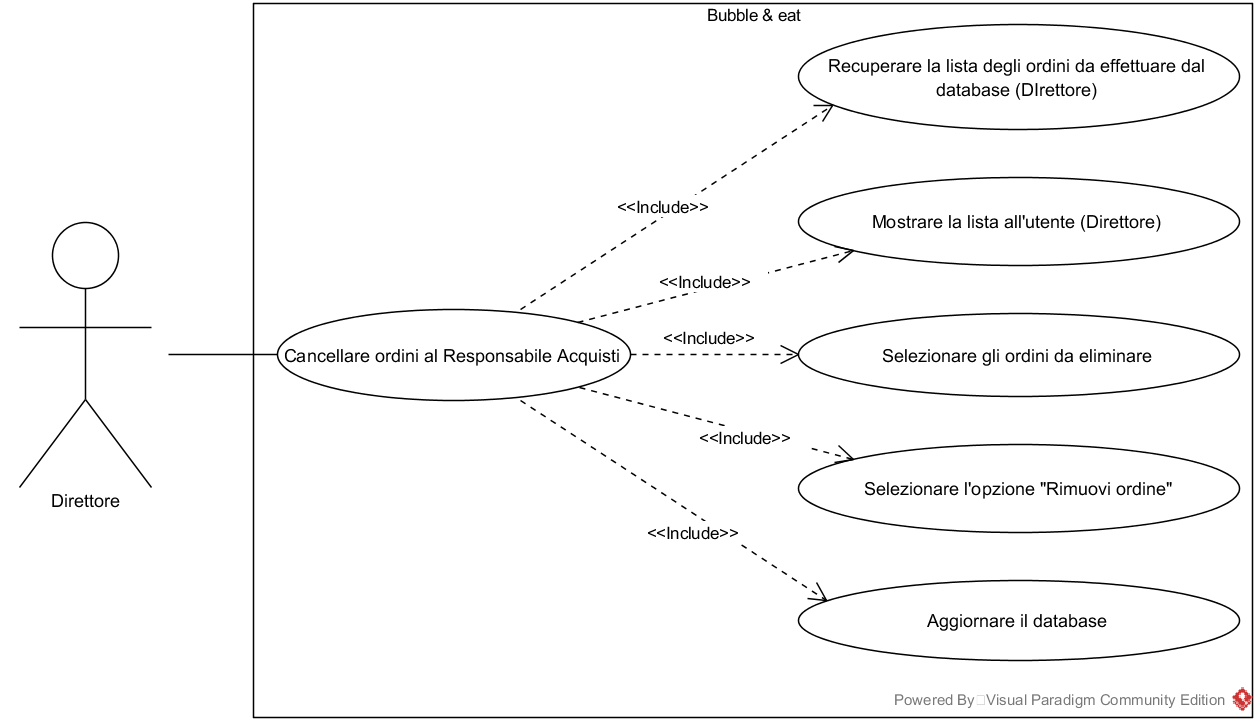
\includegraphics[width=15cm]{../../documenti/AnalisiDeiRequisiti/Diagrammi_img/uc3_15.png}
	\caption{\UCCaption{} Cancellare ordini al Responsabile Acquisti}
\end{figure}

\begin{itemize}
	\item \textbf{Attori:}
	\\Direttore.
	\item \textbf{Scopo e descrizione:} 
	\\Lo scopo di questa funzione è permettere al Direttore di eliminare ordini dalla to-do list del Responsabile Acquisti.
	\item \textbf{Precondizioni:}
	\begin{itemize}
		\item Avere Rocket.Chat;
		\item Avere la bubble del ristorante selezionato;
		\item Avere accesso alla bubble con il ruolo di Direttore.
	\end{itemize}
	\item \textbf{Flusso principale degli eventi:}
	\begin{itemize}
		\item Il Direttore seleziona la parte corrispondente della bubble;
		\item I dati vengono recuperati dal database \ref{UC3.15.1};
		\item Viene mostrata la lista degli ordini all'utente \ref{UC3.15.2};
		\item Il Direttore seleziona dalla lista gli ordini che si desidera rimuovere \ref{UC3.15.3};
		\item Il Direttore seleziona l'opzione per rimuovere gli ordini selezionati \ref{UC3.15.4};
		\item Viene aggiornato il database \ref{UC3.15.5}.
	\end{itemize}
	\item \textbf{Post-condizione:}
	\\Il Direttore ha eliminato gli elementi desiderati dalla to-do list del Responsabile Acquisti.
\end{itemize}

\UCF{Recuperare la lista degli ordini da effettuare dal database (Direttore)}{UC3.15.1}

\begin{itemize}
	\item \textbf{Attori:}
	\\Direttore.
	\item \textbf{Scopo e descrizione:} 
	\\Lo scopo di questa funzione è recuperare le informazioni sulla lista di ordini da effettuare dal database.
	\item \textbf{Precondizioni:}
	\begin{itemize}
		\item Avere Rocket.Chat;
		\item Avere la bubble del ristorante selezionato;
		\item Avere accesso alla bubble con il ruolo di Direttore.
	\end{itemize}
	\item \textbf{Flusso principale degli eventi:}
	\\I dati sugli ordini da effettuare devono essere prelevati dal database.
	\item \textbf{Post-condizione:}
	\\I dati sono prelevati dal database.
\end{itemize}

\UCF{Mostrare la lista all'utente (Direttore)}{UC3.15.2}

\begin{itemize}
	\item \textbf{Attori:}
	\\Direttore.
	\item \textbf{Scopo e descrizione:} 
	\\Lo scopo di questa funzione è permettere al Direttore di visualizzare la lista degli ordini da effettuare.
	\item \textbf{Precondizioni:}
	\begin{itemize}
		\item Avere Rocket.Chat;
		\item Avere la bubble del ristorante selezionato;
		\item Avere accesso alla bubble con il ruolo di Direttore.
	\end{itemize}
	\item \textbf{Flusso principale degli eventi:}
	\\Il Direttore deve visualizzare la lista degli ordini da effettuare.
	\item \textbf{Post-condizione:}
	\\La lista è visualizzata.
\end{itemize}

\UCF{Selezionare ordini da eliminare}{UC3.15.3}

\begin{itemize}
	\item \textbf{Attori:}
	\\Direttore.
	\item \textbf{Scopo e descrizione:} 
	\\Lo scopo di questa funzione è permettere al Direttore di selezionare che ordini eliminare.
	\item \textbf{Precondizioni:}
	\begin{itemize}
		\item Avere Rocket.Chat;
		\item Avere la bubble del ristorante selezionato;
		\item Avere accesso alla bubble con il ruolo di Direttore;
		\item La lista degli ordini da effettuare è visualizzata.
	\end{itemize}
	\item \textbf{Flusso principale degli eventi:}
	\\Il Direttore seleziona l'opzione per rimuovere un ordine.
	\item \textbf{Post-condizione:}
	\\Il Direttore ha selezionato gli ordini che desidera eliminare.
\end{itemize}

\UCF{Selezionare l'opzione \virgolette{Rimuovi ordine}}{UC3.15.4}

\begin{itemize}
	\item \textbf{Attori:}
	\\Direttore.
	\item \textbf{Scopo e descrizione:} 
	\\Lo scopo di questa funzione è permettere al Direttore di selezionare l'opzione per rimuovere ordini dalla to-do list del Responsabile Acquisti.
	\item \textbf{Precondizioni:}
	\begin{itemize}
		\item Avere Rocket.Chat;
		\item Avere la bubble del ristorante selezionato;
		\item Avere accesso alla bubble con il ruolo di Direttore;
		\item La lista degli ordini da effettuare è visualizzata;
		\item Sono selezionati ordini per la rimozione.
	\end{itemize}
	\item \textbf{Flusso principale degli eventi:}
	\\Il Direttore seleziona l'opzione per rimuovere gli ordini.
	\item \textbf{Post-condizione:}
	\\Il Direttore ha confermato l'eliminazione degli elementi selezionati.
\end{itemize}

\UCF{Aggiornare il database}{UC3.15.5}

\begin{itemize}
	\item \textbf{Attori:}
	\\Direttore.
	\item \textbf{Scopo e descrizione:} 
	\\Lo scopo di questa funzione è quello di aggiornare il database con gli ordini rimossi dal Direttore dalla lista degli acquisti.
	\item \textbf{Precondizioni:}
	\begin{itemize}
		\item Avere Rocket.Chat;
		\item Avere la bubble del ristorante selezionato;
		\item Avere accesso alla bubble con il ruolo di Direttore;
		\item Aver eliminato degli ordini.
	\end{itemize}
	\item \textbf{Flusso principale degli eventi:}
	\\Il database deve essere aggiornato con gli elementi rimossi dal Direttore dalla to-do list del Responsabile Acquisti.
	\item \textbf{Post-condizione:}
	\\Il database è aggiornato.
\end{itemize}
